\documentclass[11pt]{article}
\usepackage{graphicx}  % Include figure files
\usepackage{amsmath}
\usepackage{hyperref}

\begin{document}
\title{HCal analysis and efficiency}

\maketitle

\section*{Quasi-elastic analysis with GMn apparatus}

As discussed in the proposal, the relevant variables to select the quasi-elastic $e-N$ scattering from the resonant $e-N$ scattering are the missing mass $W^2 = M_{N}^2+2M_{N}^{2}(E-E')-Q^2$, evaluated with the BigBite resolution, of the system N$(e, e')X$, and the transverse missing momentum.
Figure~\ref{fig:W2} displays the event distributions in $W^2$ for both our simulated quasi-elastic and inelastic samples within the following set of fiducial acceptance cuts:
%
\begin{itemize}
\item{the electron track is reconstructed in BigBite;}
\item{the total energy deposited in the BigBite calorimeter is above the 3 GeV threshold for an average 4.2 GeV elastic peak (for $\epsilon = 0.84$ kinematic);}
\item{the electron track must fire at least 3 PMTs in the GRINCH detectors;}
\item{the total energy deposited in HCal is above the 0.10 GeV threshold. This corresponds to 90\% efficiency of the 3.2 GeV/c nucleons which deposit 0.20 GeV in the HCal (scintillator material).}
\end{itemize}
%
%According to $^3$, %\footnote{Phys.~Rev.~C81.055213, https://arxiv.org/abs/0712.3731},
%the fit residue to the data between 4 and 6 GeV fluctuates by $\pm$ 10\%. We assume a 20\% systematic error attached on our inelastic background estimation.% or 0.4\% relative quasi-elastic.\\
%
\begin{figure}[h]
  \centering
    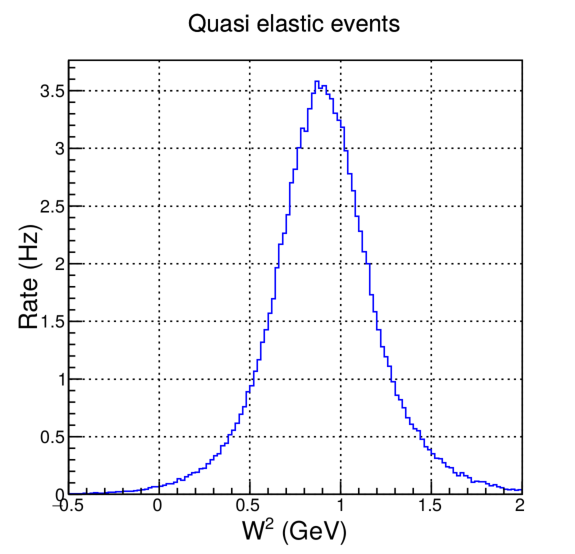
\includegraphics[width=5cm]{W2_sig.pdf}
    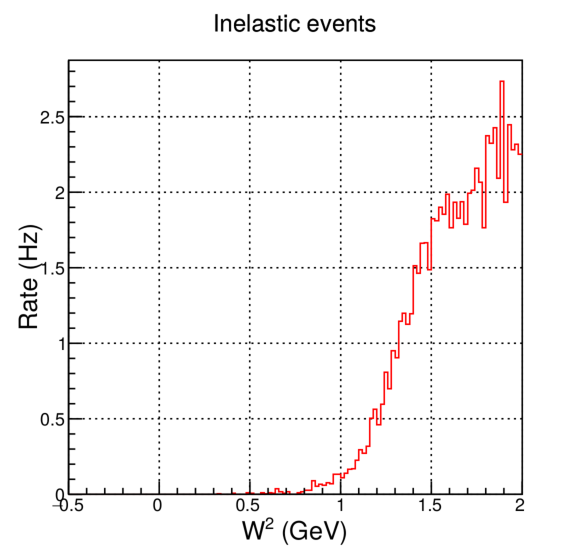
\includegraphics[width=5cm]{W2_inel.pdf}
    \caption{Event distributions in $W^2 = M_{N}^2+2M_{N}^{2}(E-E')-Q^2$  for quasi elastic $e-N$ (left) and inelastic resonant $e-N$ (right) within the fiducial analysis cuts.}
    \label{fig:W2}
\end{figure}
%

Before reconstructing the nucleon momentum, it is necessary to apply a selection cut on $W^2$ to reject a fraction of the inelastic events. To this end, only events for which $W^2<1.10~{\rm GeV}^2$ are selected for further discussion. Within this selection, our total number of events counts 97\% of quasi-elastic and 3\% of inelastic.
% this cut is 76\% for quasi-elastic and 1\% for inelastic.

Now we will discuss the missing perpendicular momentum.
The nucleon momentum and direction is reconstructed using the position of the HCal cluster, on the first step {\em under the assumption that it is a neutron}.
We use the direction of the virtual photon vector $\vec{q}$ (corrected with the vertex position) to project the expected neutron position.
The difference between the reconstructed and the projected nucleon position is shown, projected on $x$ (the non-dispersive direction) and $y$ (the dispersive direction), for both quasi-elastic and inelastic events on figure~\ref{hcal_id_2D}.
%
\begin{figure}[!h]
  \centering
    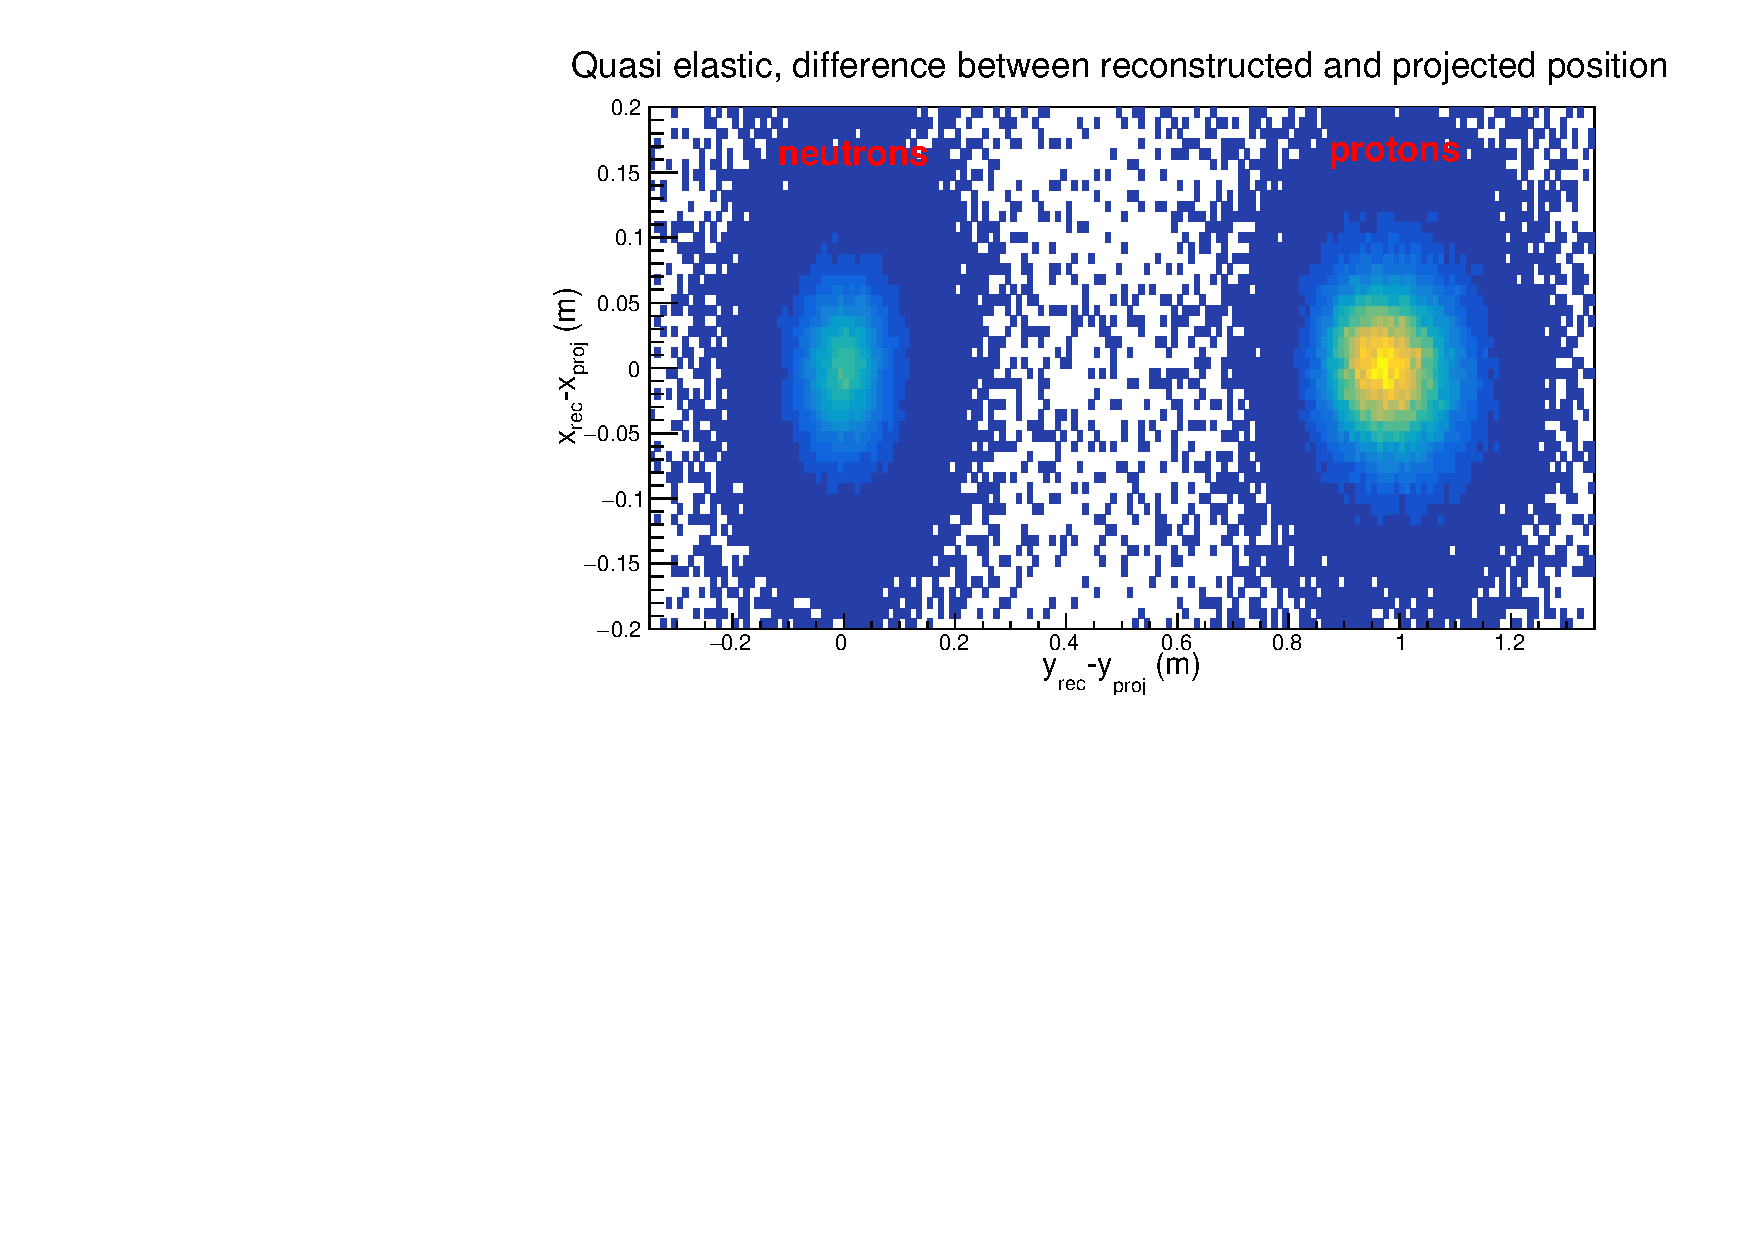
\includegraphics[width=6cm]{HCal_PID_QE.pdf}
    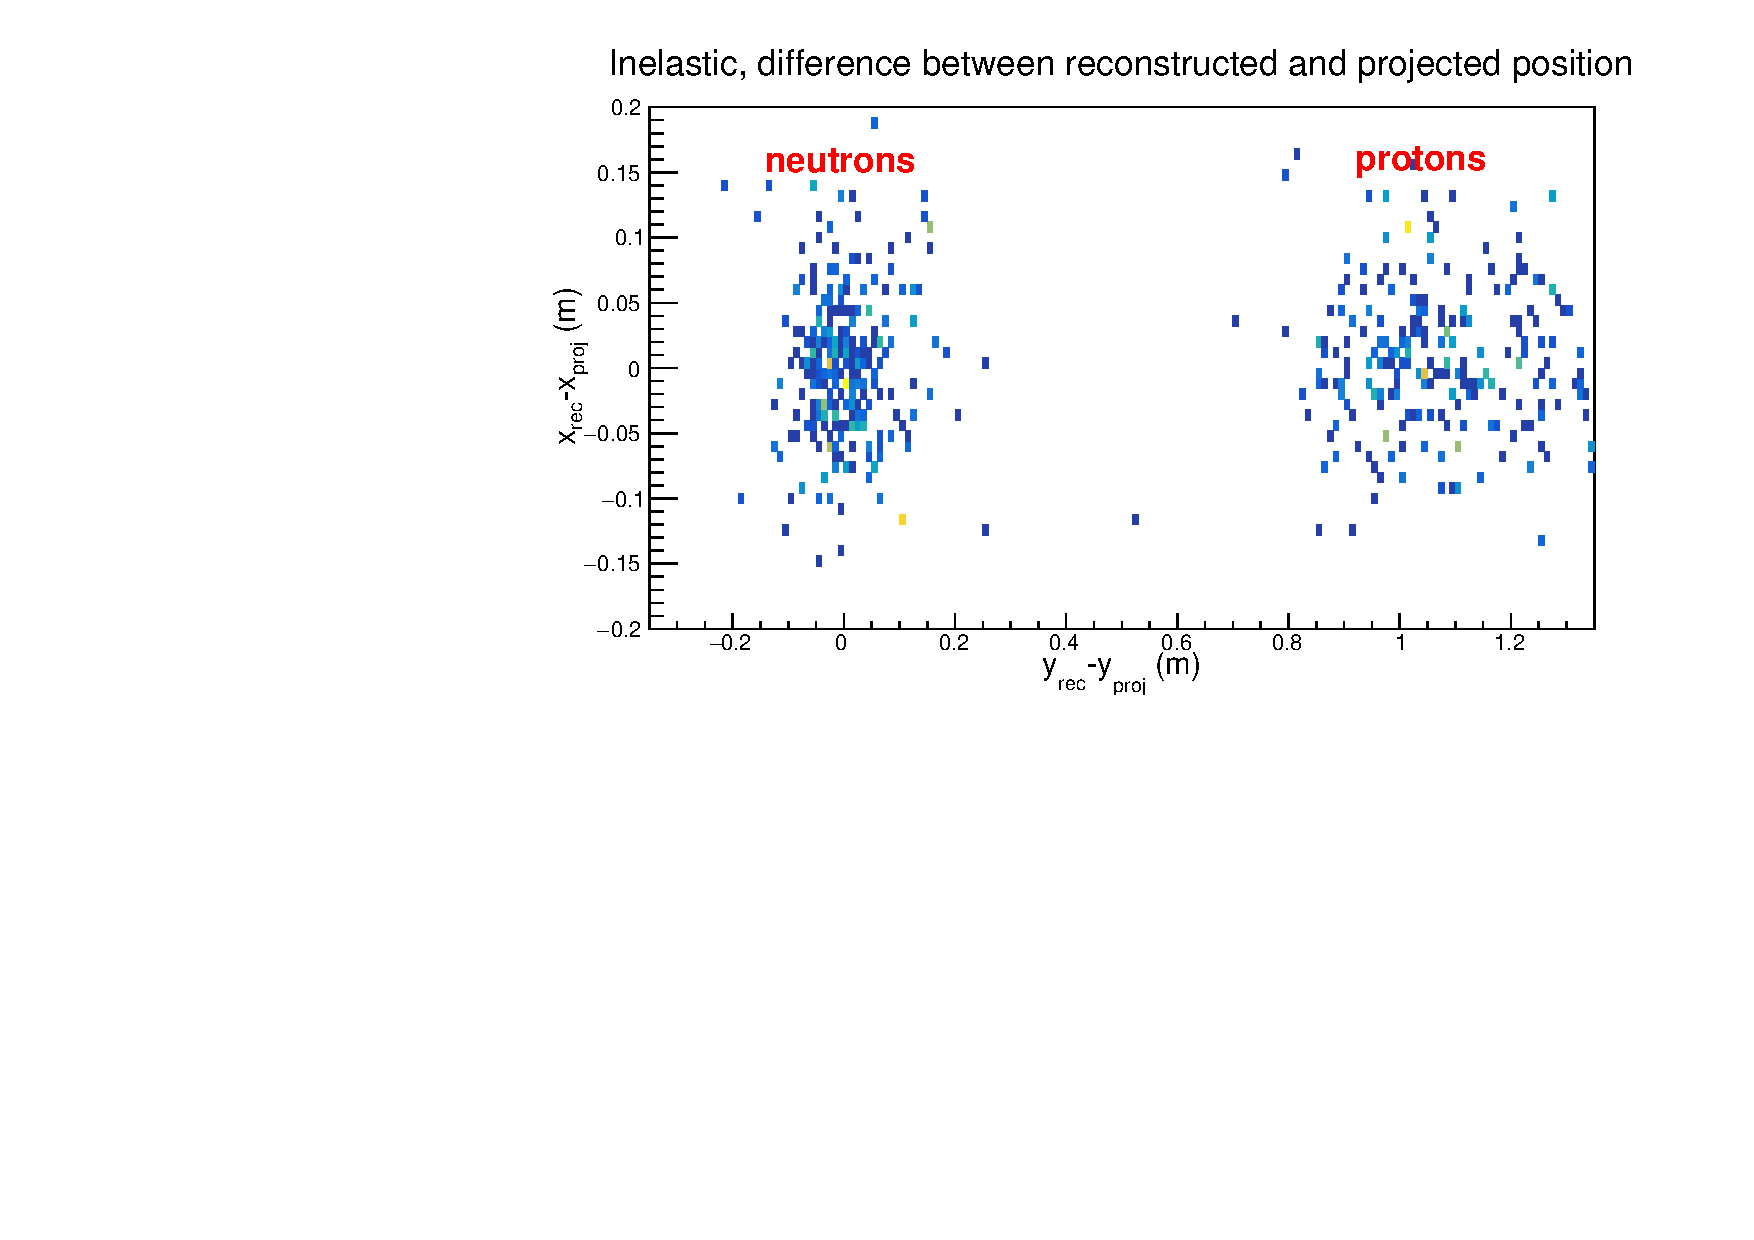
\includegraphics[width=6cm]{HCal_PID_Inel.pdf}
    \caption{Difference of projected position and reconstructed position for the nucleons in $x$ (non-dispersive direction) and $y$ (dispersive direction), for quasi-elastic events (left) and inelastic events (right). On each plot We clearly notice two structures. The structure on the left, centered at 0, is due to the neutrons. The structure on the right, shifted by about 1~m is due to the protons, which are deflected upwards by the magnetic field. 
    }
    \label{hcal_id_2D}
\end{figure}
%
We clearly distinguish in each case two structures, one which can be identified a the neutrons, centered on zero in both $x$ and $y$, and one which can be identified as the protons, which are deflected upwards and are shifted by about 1~m in $y$.
Figure~\ref{hcal_id_y} also shows the difference between the reconstructed and the projected nucleon position, except projected on $y$ (the dispersive direction), for both the quasi-elastic and inelastic events. Comparing both the expected inelastic and elastic yields in this variable side-by-side evidences further the important role of the $W^2<1.10~{\rm GeV}^2$ selection to filter out inelastic events. 
%
\iffalse
\begin{figure}[!h]
  \centering
    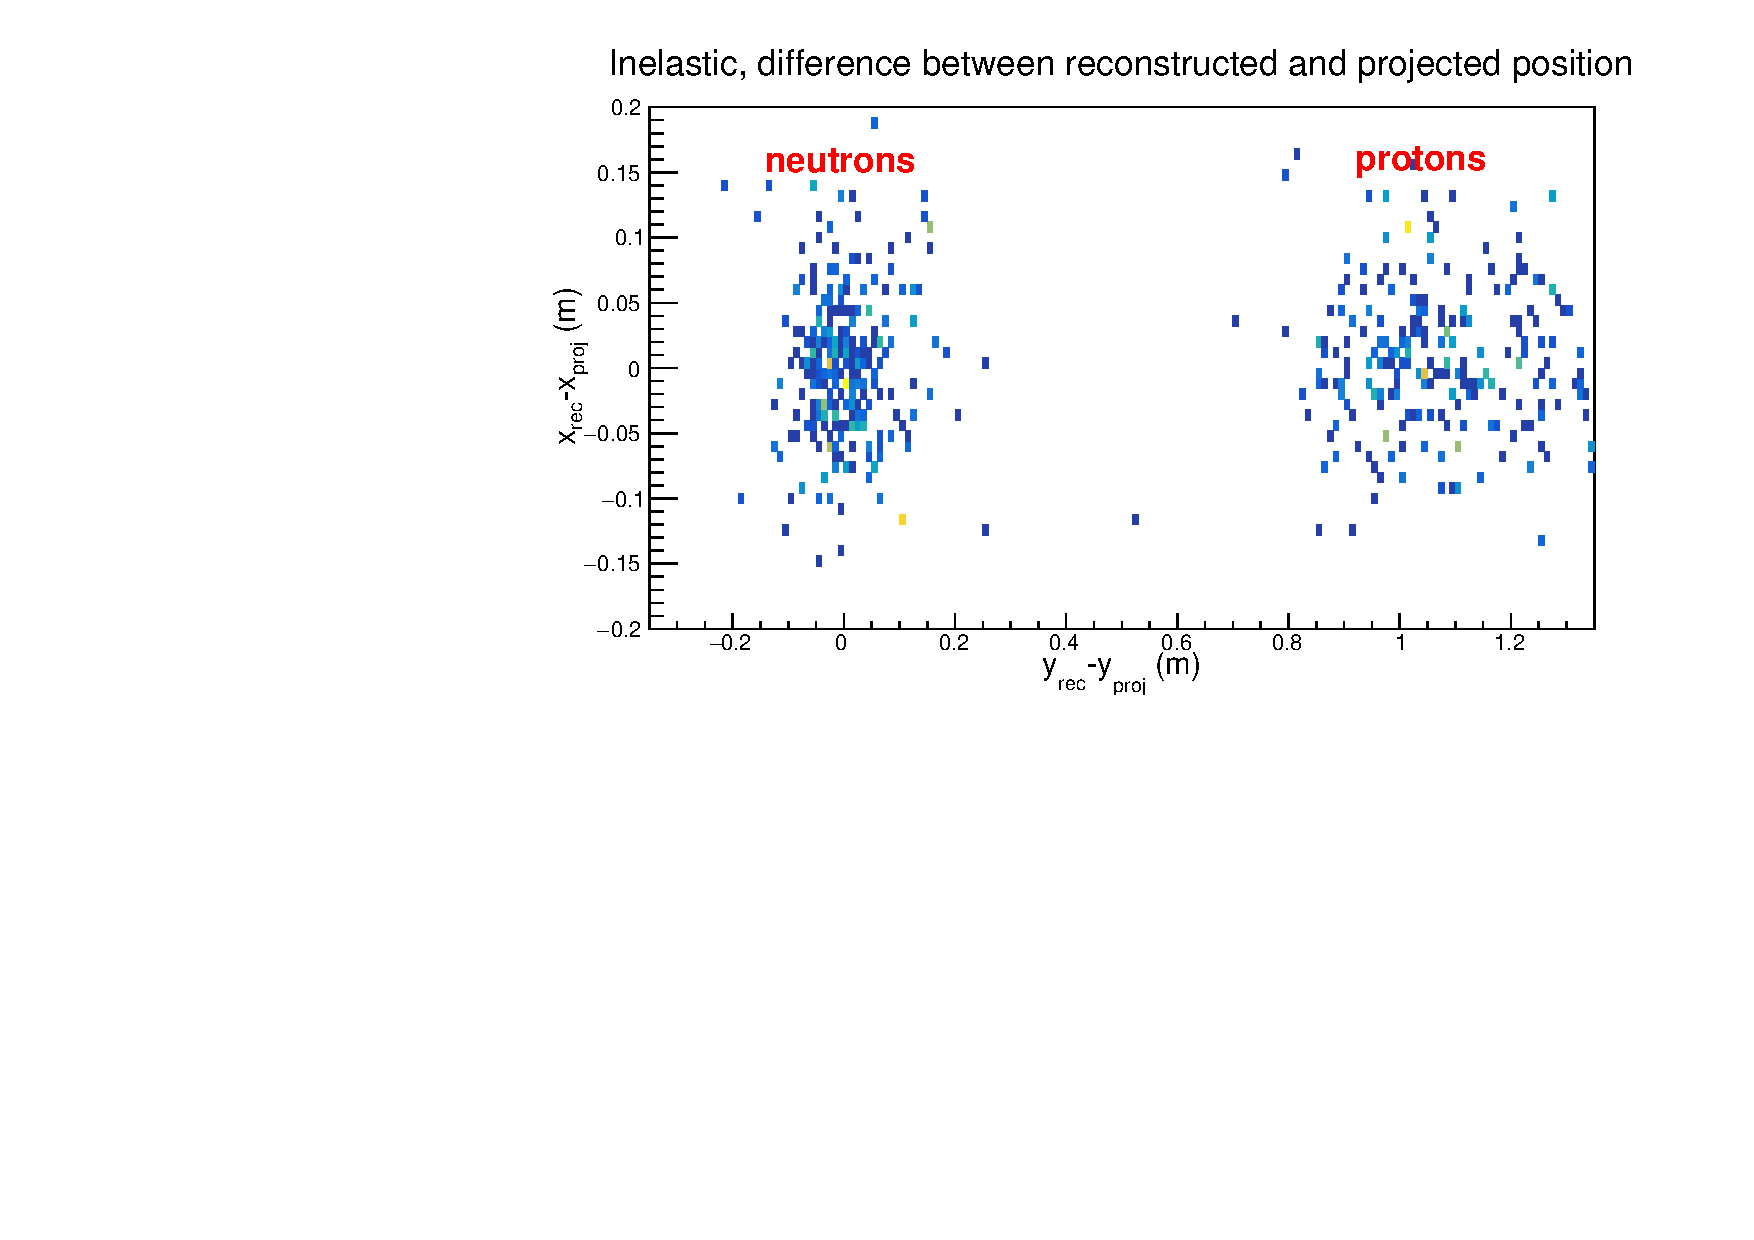
\includegraphics[width=10cm]{HCal_PID_Inel.pdf}
    \caption{Difference of projected position and reconstructed position for the nucleons in $x$ (non-dispersive direction) and $y$ (dispersive direction), for inelastic events. The selection for these distributions are the fiducial cuts $W^2<1.10~{\rm GeV}^2$. We clearly notice two structures. The structure on the left, centered at 0, is due to the neutrons. The structure on the right, shifted by about 1~m is due to the protons, which are deflected upwards by the magnetic field. 
    }
    \label{hcal_id_inel}
\end{figure}
\fi
%
\begin{figure}[!h]
  \centering
    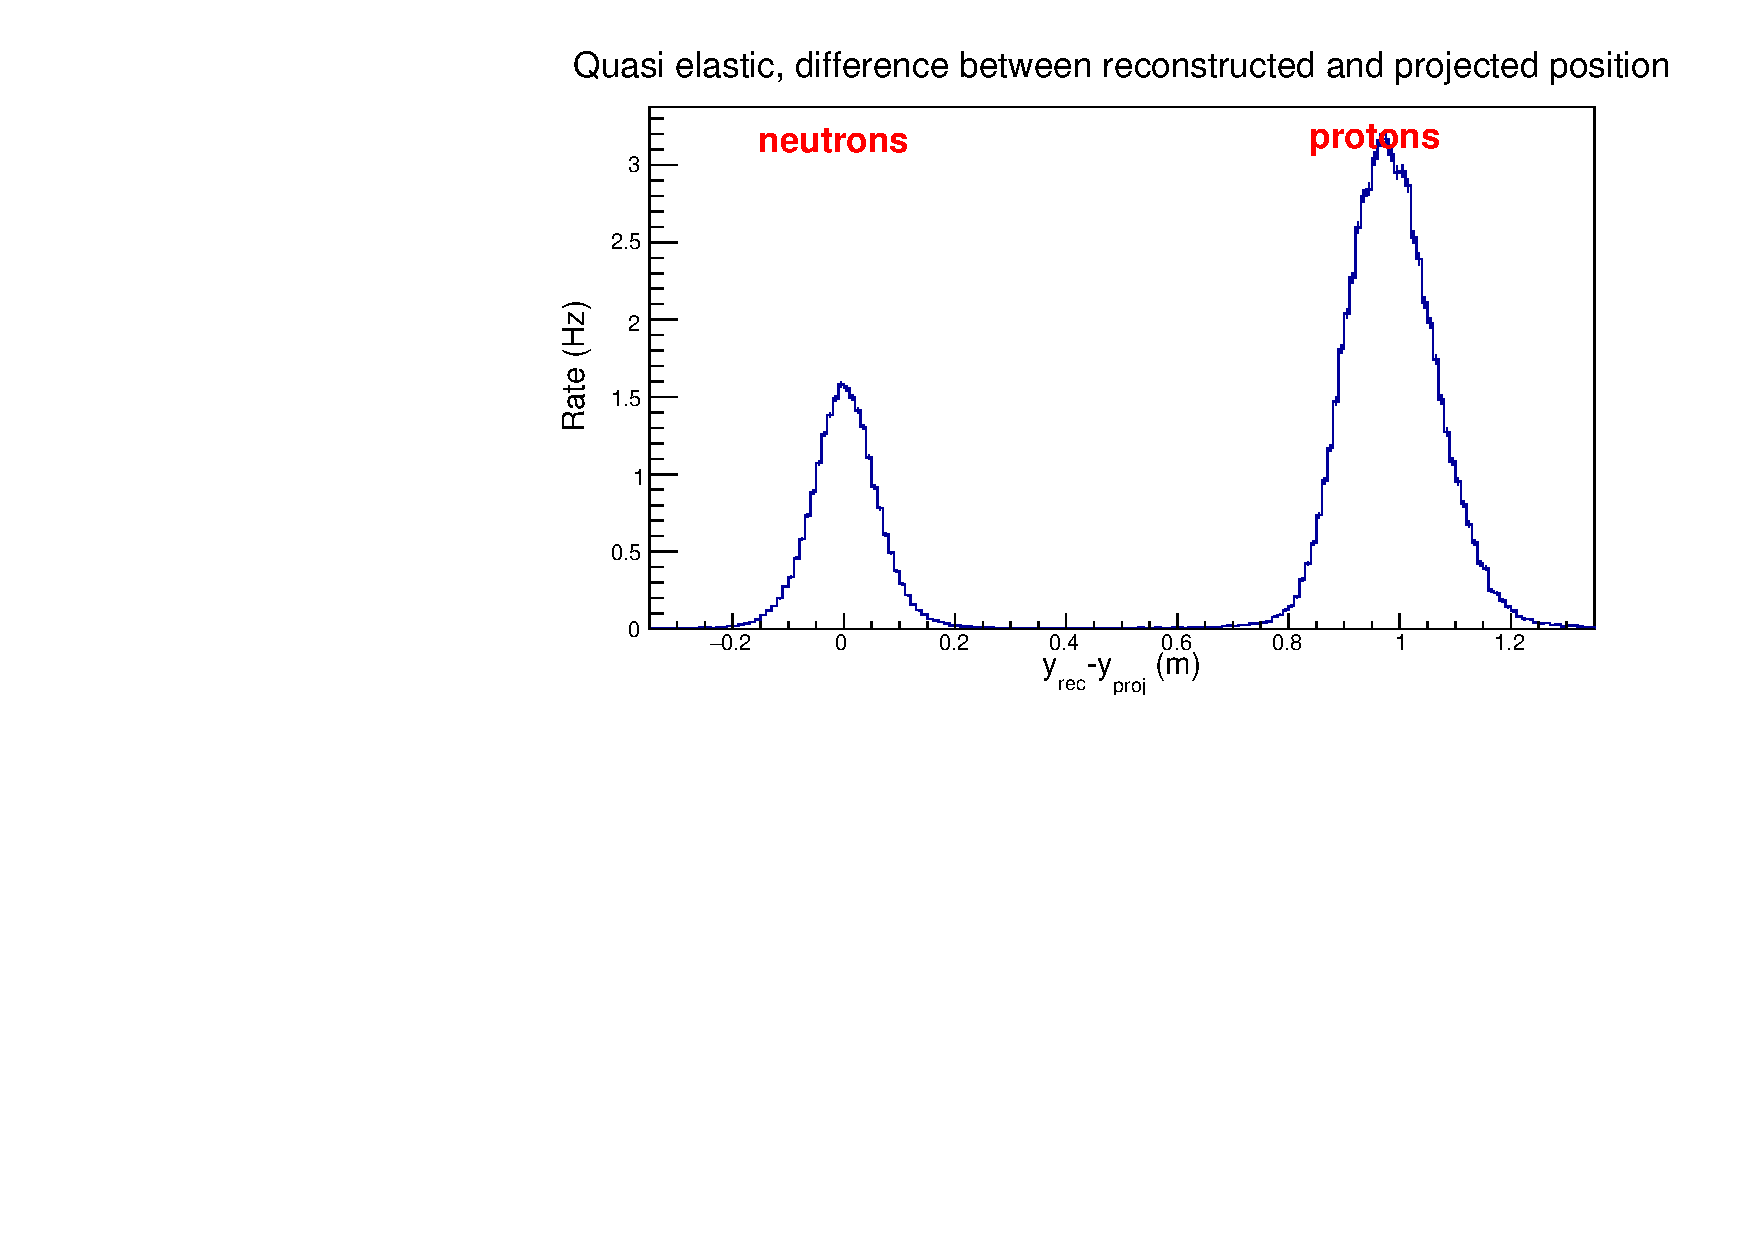
\includegraphics[width=6cm]{HCal_PID_QE_y.pdf}
    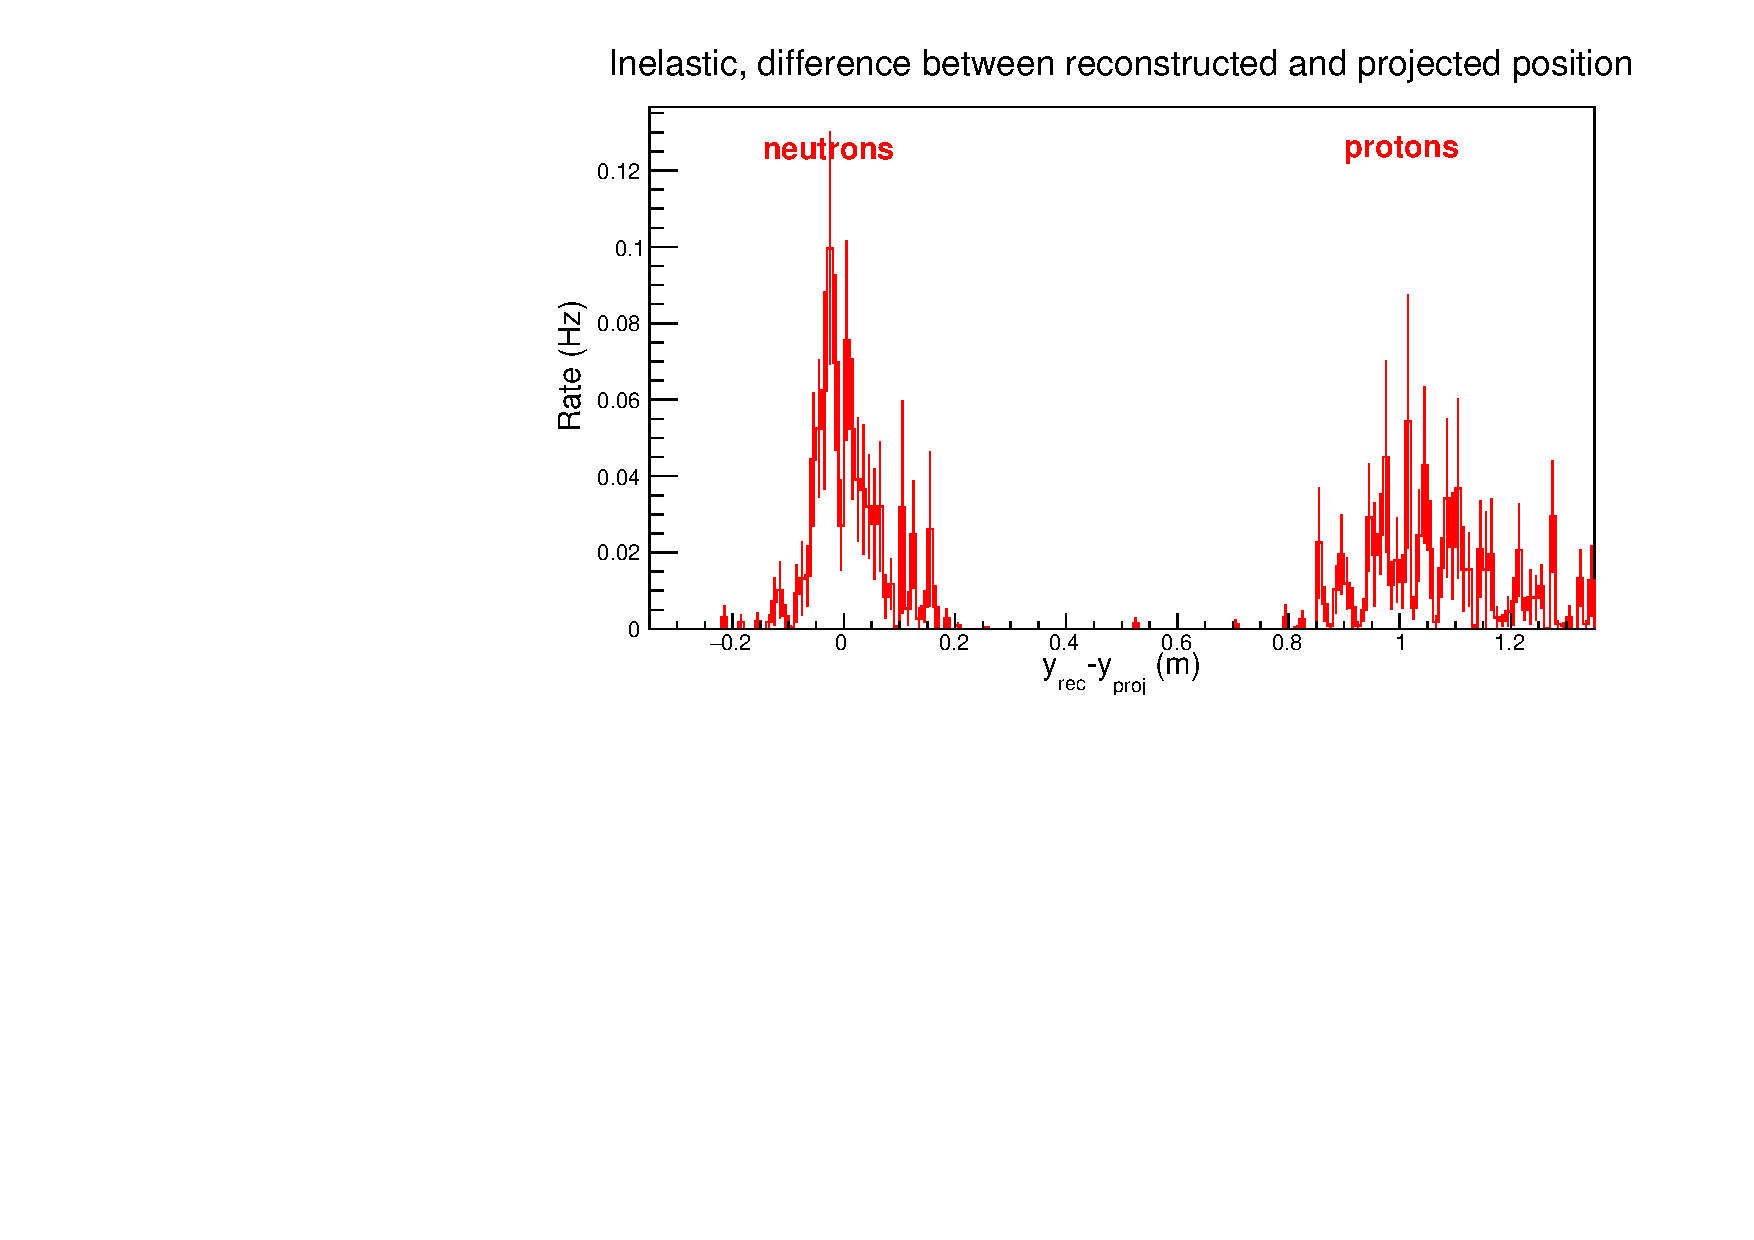
\includegraphics[width=6cm]{HCal_PID_Inel_y.pdf}
    \caption{Difference of projected position and reconstructed position for the nucleons projected in $y$ (dispersive direction), compared between quasi-elastic (left) and inelastic (right) events. The selection for these distributions are the fiducial cuts $W^2<1.10~{\rm GeV}^2$. We may notice that the selection on $W^2<1.10~{\rm GeV}^2$ already reduces drastically the proportion of inelastic with respect to quasi elastic. We may also see that the distribution for the proton is slightly wider. %, which will induce a slight decrease in $e-p$ events, which is fully calculable.
    }
    \label{hcal_id_y}
\end{figure}
%

As a second step, for the nucleons identified as protons (based on the location of the HCal cluster position with respect to its projected position), we need to correct the HCal reconstructed position $y_{rec}$ by the average shift $\Delta y_{p, avg}$ observed in figure~\ref{hcal_id_2D} for the nucleons identified as protons.

%Then, the HCal cluster position can be combined with the vertex position to retrieve the nucleon scattering angle $\theta_N$.
The nucleon momentum norm $p' = |\vec{p'}|$ is assumed to be equal to the virtual photon norm $|\vec{q}|$.
With this information we can calculate the proton shift $\Delta y_{p}$ for each proton.
%evaluated assuming the elastic scattering on a free nucleon, using the relation between the nucleon scattering angle and momentum in elastic scattering: $\vec{q}$
%$p' = 2M_N E (M_n+E cos(\theta_N)/(M_N^2+2M_N E+(E \sin{\theta_N}^2)$, with $E$ the beam energy and $M_N$ the nucleon mass.

With this information we may build the transverse components of the nucleon momentum (in the SBS coordinates system) $p'_{x, SBS}$ and $p'_{y, SBS}$.
For both the protons and neutrons, $p'_{x, SBS}$ can be written as $p'_{x, SBS} = p' \times (x_{rec}-v\sin{\theta_{SBS}})/(D_{HCal}-v\cos{\theta_{SBS}})$ (with $v$ the reconstructed vertex position, $D_{HCal}$ the HCal distance to the target and $\theta_{SBS}$ the spectrometer angle.
For the neutrons, $p'_{y, SBS}$ is $p'_{y, SBS} = p' \times y_{rec}/(D_{HCal}-v\cos{\theta_{SBS}})$.
For the protons, $p'_{y, SBS}$ must be written as $p'_{y, SBS} = p' \times (y_{rec} - \Delta y_{p})/(D_{HCal}-v\cos{\theta_{SBS}})$.

The nucleon momentum components in the SBS coordinates system $p'_{x, SBS}$ and $p'_{y, SBS}$ can then be transformed (using the corrected HCal distance to the target $D_{HCal}-v\cos{\theta_{SBS}}$) into the nucleon momentum components in the Hall~A coordinate system $p'_{x}$, $p'_y$ and $p'_z$, with the best resolution achievable. 

In Hall~A coordinate system, using the nucleon meomentum combined with the virtual photon vector $\vec{q}$, we may reconstruct the transverse missing momentum $p_{_{\perp} miss} = \sqrt{(q_{x}-p'_{x})^2+(q_{y}-p'_{y})^2}$, which is another very powerful variable to reject more inelastic background.
Figure~\ref{fig:pperp} displays the event distributions in $p_{_{\perp} miss}$ for our simulated quasi-elastic sample within our fiducial acceptance cuts%, but before requiring $W^2<1.10~{\rm GeV}^2$.
, and requiring $W^2<1.10~{\rm GeV}^2$.
%
\begin{figure}[h]
  \centering
    %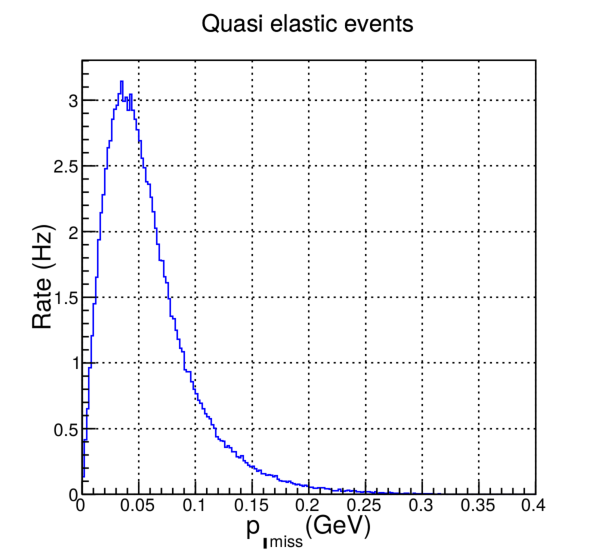
\includegraphics[width=5cm]{pperp_sig.pdf}
    %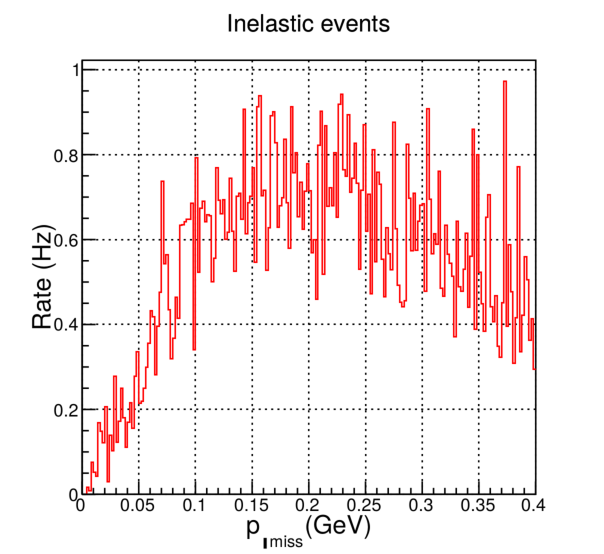
\includegraphics[width=5cm]{pperp_inel.pdf}
    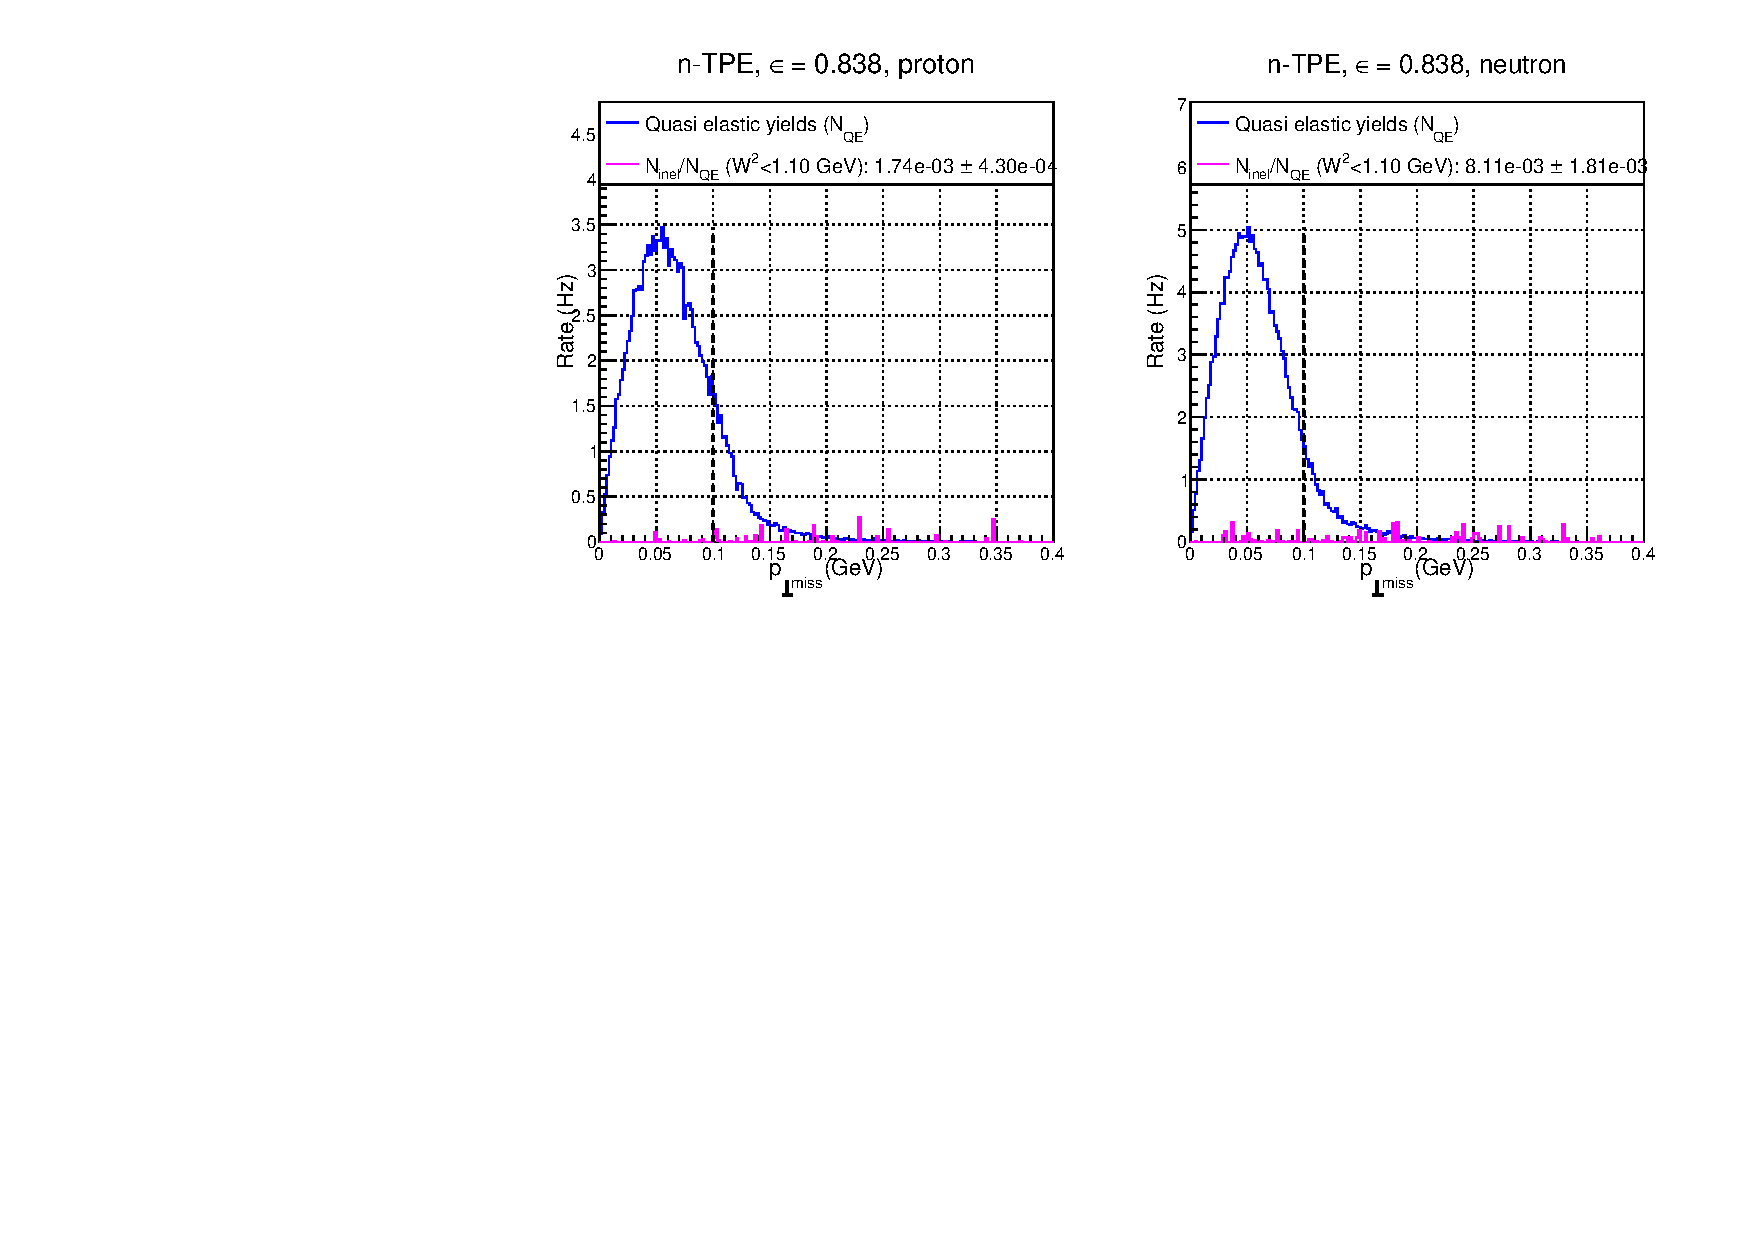
\includegraphics[width=12cm]{gen-tpe_he_pperp_acc_real_new.pdf}
    %\caption{Event distributions in $p_{_{\perp} miss} = \sqrt{(q_{x}-p'_{x})^2+(q_{y}-p'_{y})^2}$ for quasi elastic $e-N$ (left) and inelastic resonant $e-N$ (right) within the fiducial analysis cuts, but before requiring $W^2<1.10~{\rm GeV}^2$.}
    \caption{Compared quasi-elastic (blue) and inelastic (magenta) distributions for $p_{_{\perp} miss} = \sqrt{(q_{x}-p'_{x})^2+(q_{y}-p'_{y})^2}$, within fiducial analysis cuts, after requiring $W^2<1.10~{\rm GeV}^2$, for the high $\epsilon$ kinematic, separated between protons on the left and neutrons on the right). The inelastic contamination of quasi-elastic events and their error bars are quoted in the legends.}
    \label{fig:pperp}
\end{figure}
%
%After applying $W^2<1.10~{\rm GeV}^2$ 
After selection on $W^2 <1.10 {\rm GeV}^2$ and $p_{_{\perp} miss} <0.1$~GeV, the inelastic contamination of our quasi-elastic sample is better than 1\%, with 0.2\% systematic uncertainties.

The nucleon time-of-flight information can also be used to further suppress background. The HCal time resolution of 0.5 ns allows to resolve time-of-flight for 3.2 GeV/c nucleons with 12\% resolution.

In addition, the level of inelastic contamination reported in the document are for the en and ep yields.
The observable we are interested in is the {\it ratio} $N_{en}/N_{ep}$, in which the inelastic contribution partly cancels.
The cancellation is not complete because the fractional errors in the numerator and 
denominator will differ.
But the partial cancellation results in a fractional error on the ratio which is smaller than the fractional error contributed to the neutron or proton counts.
In addition, in the (likely) event that we underestimate our background contamination,
we expect to underestimate it by the same amount for $e-p$ and $e-n$, so the point above remains true.\\

\newpage

\section*{Experimental determination of HCal efficiency}

Simulated efficiencies were obtained from the amplitude distributions like the ones shown as in the histograms in Fig.~\ref{fig:Neff}.
For example, with threshold 100 MeV the efficiency for the proton is 90.8\% (Fig.~\ref{fig:Neff}~{\bf(a)}) Similar distribution for the neutron in Fig.~\ref{fig:Neff}~{\bf(b)} leads to 92.0\% efficiency for the same threshold.\\
The efficiency $\eta_{n}$ is calculated as the ratio of the number of events with energy deposit above 0.10 GeV over the total number of events.
%
\begin{figure}[!h]
  \centering
  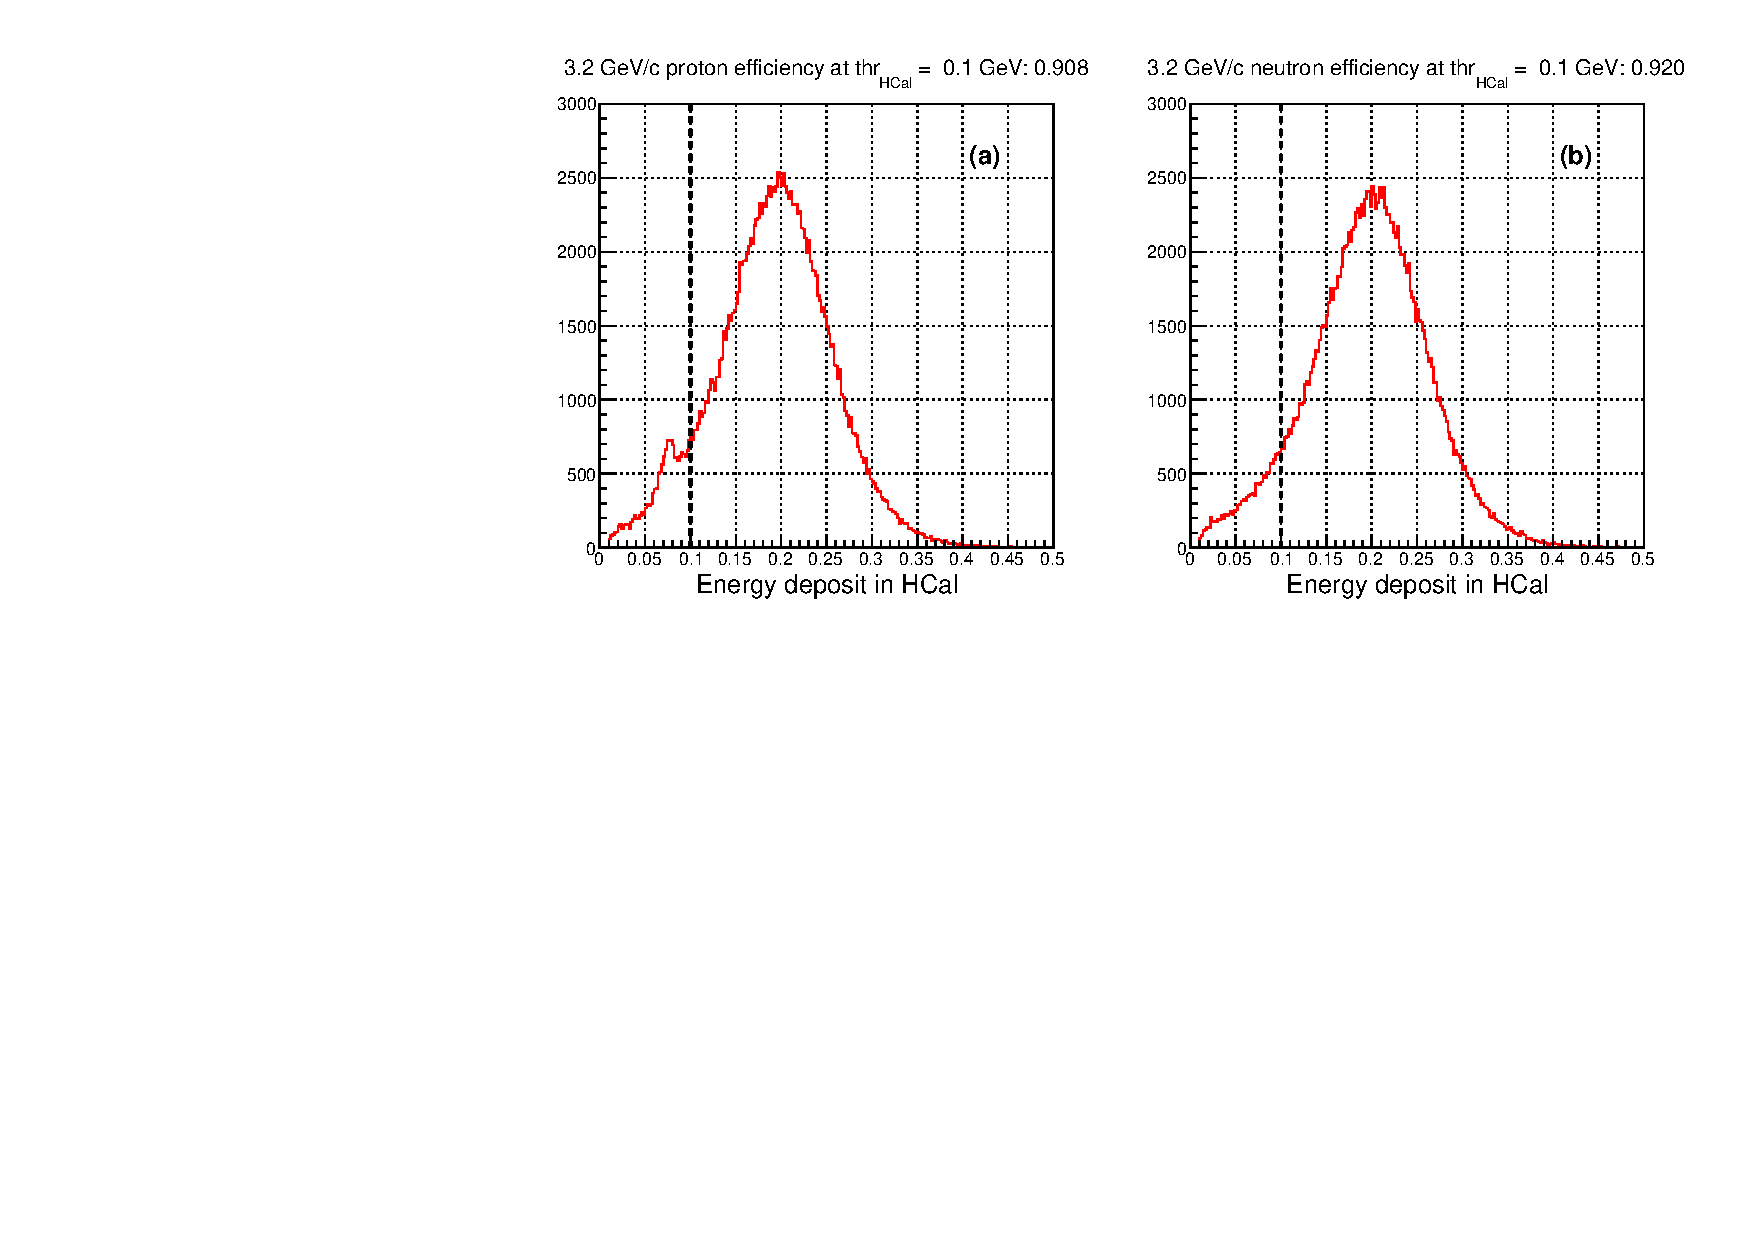
\includegraphics[width=12cm]{ProtVsNeut_MC.pdf}
  \caption{Amplitude signal expected in HCal for the protons~{\bf(a)} and the neutrons~{\bf(b)}. The efficiency is shown for a 0.1 GeV threshold.}
  \label{fig:Neff}
\end{figure}
%
%To dissipate any misunderstanding: the 90\% ``efficiency'' with 0.1 GeV quoted elsewhere (proposal, presentation) represents the fraction of quasi elastic 3.2 GeV/c nucleons which, if they deposit any energy in HCal, deposit 0.1 GeV or more. The efficiencies quoted in this document includes the small fraction of cases (about 5\%) when the nucleon does not give any signal at all.
%
%\begin{figure}[!h]
%  \centering
%  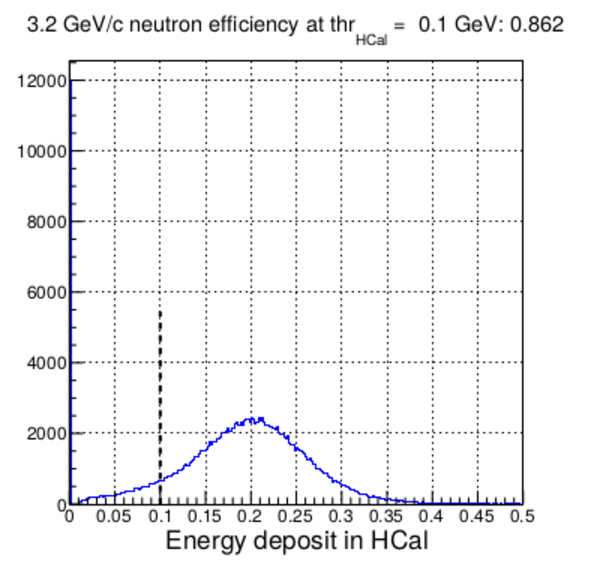
\includegraphics[width=5cm]{Neut_Eff_MC.pdf}
%  \caption{Neutron amplitude signal expected in HCal.}
%  \label{fig:neff}
%\end{figure}
%

We also would like to show how the efficiency will be measured.
This will be done by using "elastic" reactions H$(e,e’)p$, H$(\gamma,\pi^+)n$
and more with D$(\gamma,\pi^+)n$ and D$(\gamma,\pi^-)p$ single pion production.
Fig.~\ref{fig:Nproj}~{\bf(a)} shows the projected proton position from H$(e,e’)p$, 
Fig.~\ref{fig:Nproj}~{\bf(b)} shows the projected proton position from H$(\gamma,\pi^+)n$.
%
\begin{figure}[!h]
  \centering
  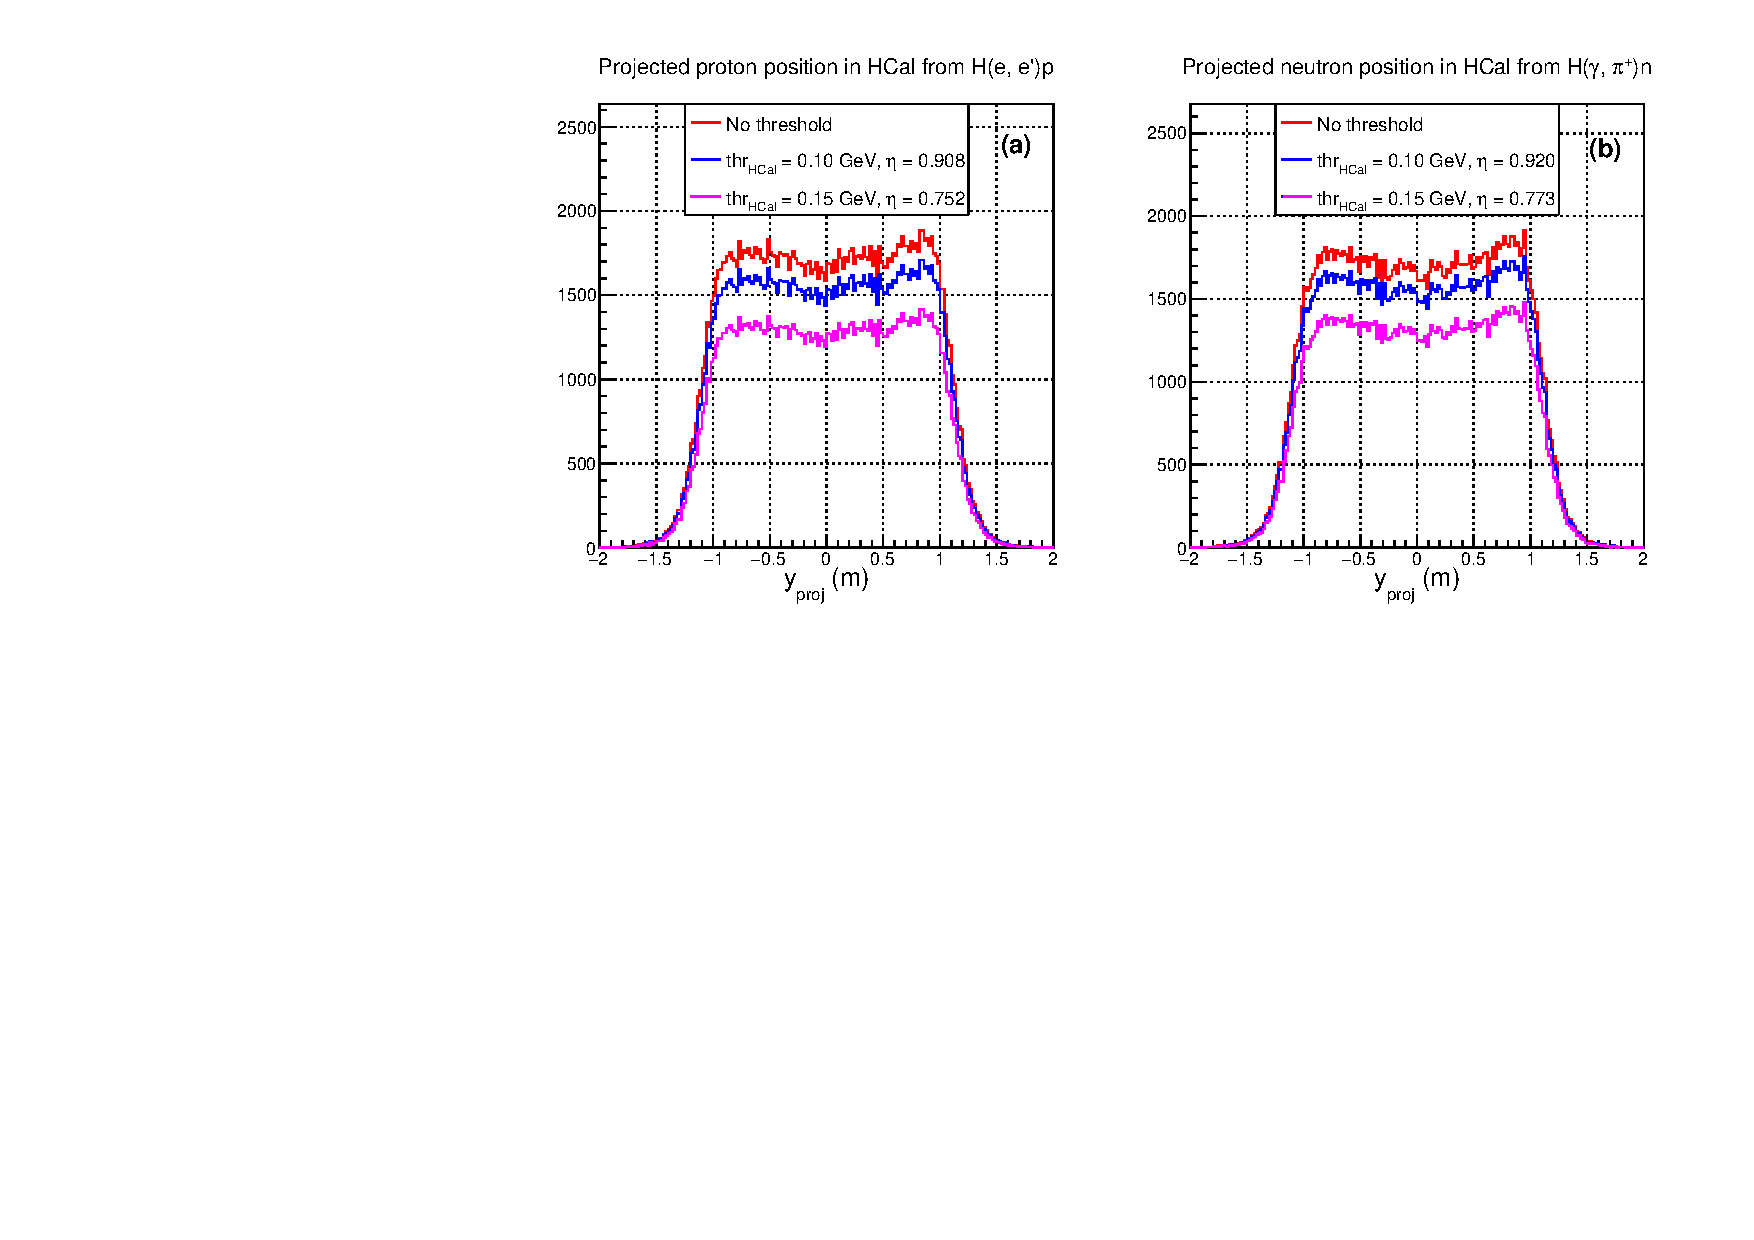
\includegraphics[width=12cm]{ProtVsNeut_CalibYproj.pdf}
  \caption{Projected position in HCal in for the protons in H$(e,e’)p$~{\bf(a)} and the neutrons in H$(\gamma,\pi^+)n$~{\bf(b)}. On both panels, red distributions show the projected distribution for $p$, $n$, not detected; blue distributions show the distribution for $p$, $n$ detected with a 0.1 GeV threshold; magenta distributions show the distribution for $p$, $n$ detected with a 0.15 GeV threshold.}
  \label{fig:Nproj}
\end{figure}
%
In each case, the trigger will not use the nucleon detector information.
Analysis will use the amplitude distribution in the same way as done on  Fig.~\ref{fig:Neff} with the red distributions.
Blue distributions on Fig.~\ref{fig:Nproj} show the expected Y distribution applying a 0.10 GeV threshold on HCal;
Magenta distributions on Fig.~\ref{fig:Nproj} show the expected Y distribution applying a 0.15 GeV threshold on HCal.
As reported in the E12-09-019 GMn proposal\footnote{https://www.jlab.org/exp\_prog/proposals/09/PR12-09-019.pdf} on Table~8, the expected recorded statistics for H$(\gamma,\pi^+)n$ are of the order of 4000 events, which will represent a relative 1.5\% uncertainty on the neutron efficiency. The recorded statistics for H$(e,e’)p$ are of the order of 82000 events, which will represent a relative 0.3\% uncertainty on the proton efficiency.\\

\section*{Impact of efficiency ratio on the neutron / proton yields ratio}

{\hskip 0.7cm}We want to evaluate the impact of the ratio of hadron efficiencies,\\
$R_{\eta_{n/p}} = \eta_n/\eta_p$
on the ratio of neutrons to proton yields $R_{n/p} = N_{en}/N_{ep}$.

To obtain the ``true'' ratio of neutrons to proton yields $R_{n/p}$ from the recorded ``raw''
ratio of neutrons to proton yields $R_{n/p, raw}$,
this ratio needs to be corrected by $R_{n/p}$.
%
\begin{equation}
  R_{n/p} = R_{n/p, raw}/R_{\eta_{n/p}}
\end{equation}
%
Hence, the uncertainty, $\Delta R_{n/p}$ of $R_{n/p}$ could be expressed as:
%
\begin{equation}
  \Delta R_{n/p}/R_{n/p} = \Delta R_{\eta_{n/p}}/R_{\eta_{n/p}}.
\end{equation}
%
To evaluate the uncertainty of $R_{\eta_{n/p}} = \eta_p/\eta_n$,
we need to account for the strong correlation between $\eta_p$ and $\eta_n$, $\rho_{\eta_{n/p}}$. 
We can define the covariance between the uncertainties $\Delta \eta_p$ and $\Delta \eta_n$,
$\sigma_{\eta_{n/p}} = \rho_{\eta_{n/p}} \Delta \eta_{n} \Delta \eta_{p}$ \footnote{https://en.wikipedia.org/wiki/Covariance\_and\_correlation}.

According to\footnote{https://www.sagepub.com/upm-data/6427\_Chapter\_4\_\_Lee\_(Analyzing)\_I\_PDF\_6.pdf}, we can write the uncertainty on the ratio efficiencies:
%\footnote{line~5 of table in https://en.wikipedia.org/wiki/Propagation\_of\_uncertainty\#Example\_formulae}

%
%\begin{equation}
\begin{align}
  \frac{\Delta R_{\eta_{n/p}}}{R_{\eta_{n/p}}} &= \sqrt{ \left( \frac{\Delta \eta_{n}}{\eta_{n}} \right)^2
    + \left( \frac{\Delta \eta_{p}}{\eta_{p}} \right)^2
    - 2 \frac{\sigma_{\eta_{n/p}}}{\eta_{n}\eta_{p}} }
  \\
  &= \sqrt{ \left( \frac{\Delta \eta_{n}}{\eta_{n}} \right)^2
    + \left( \frac{\Delta \eta_{p}}{\eta_{p}} \right)^2
    - 2 \frac{\rho_{\eta_{n/p}} \Delta\eta_{n} \Delta\eta_{p}}{\eta_{n}\eta_{p}} }
  \label{eq:uncert_exact}
  %\end{equation}
\end{align}
%
\begin{figure}[!h]
  \centering
  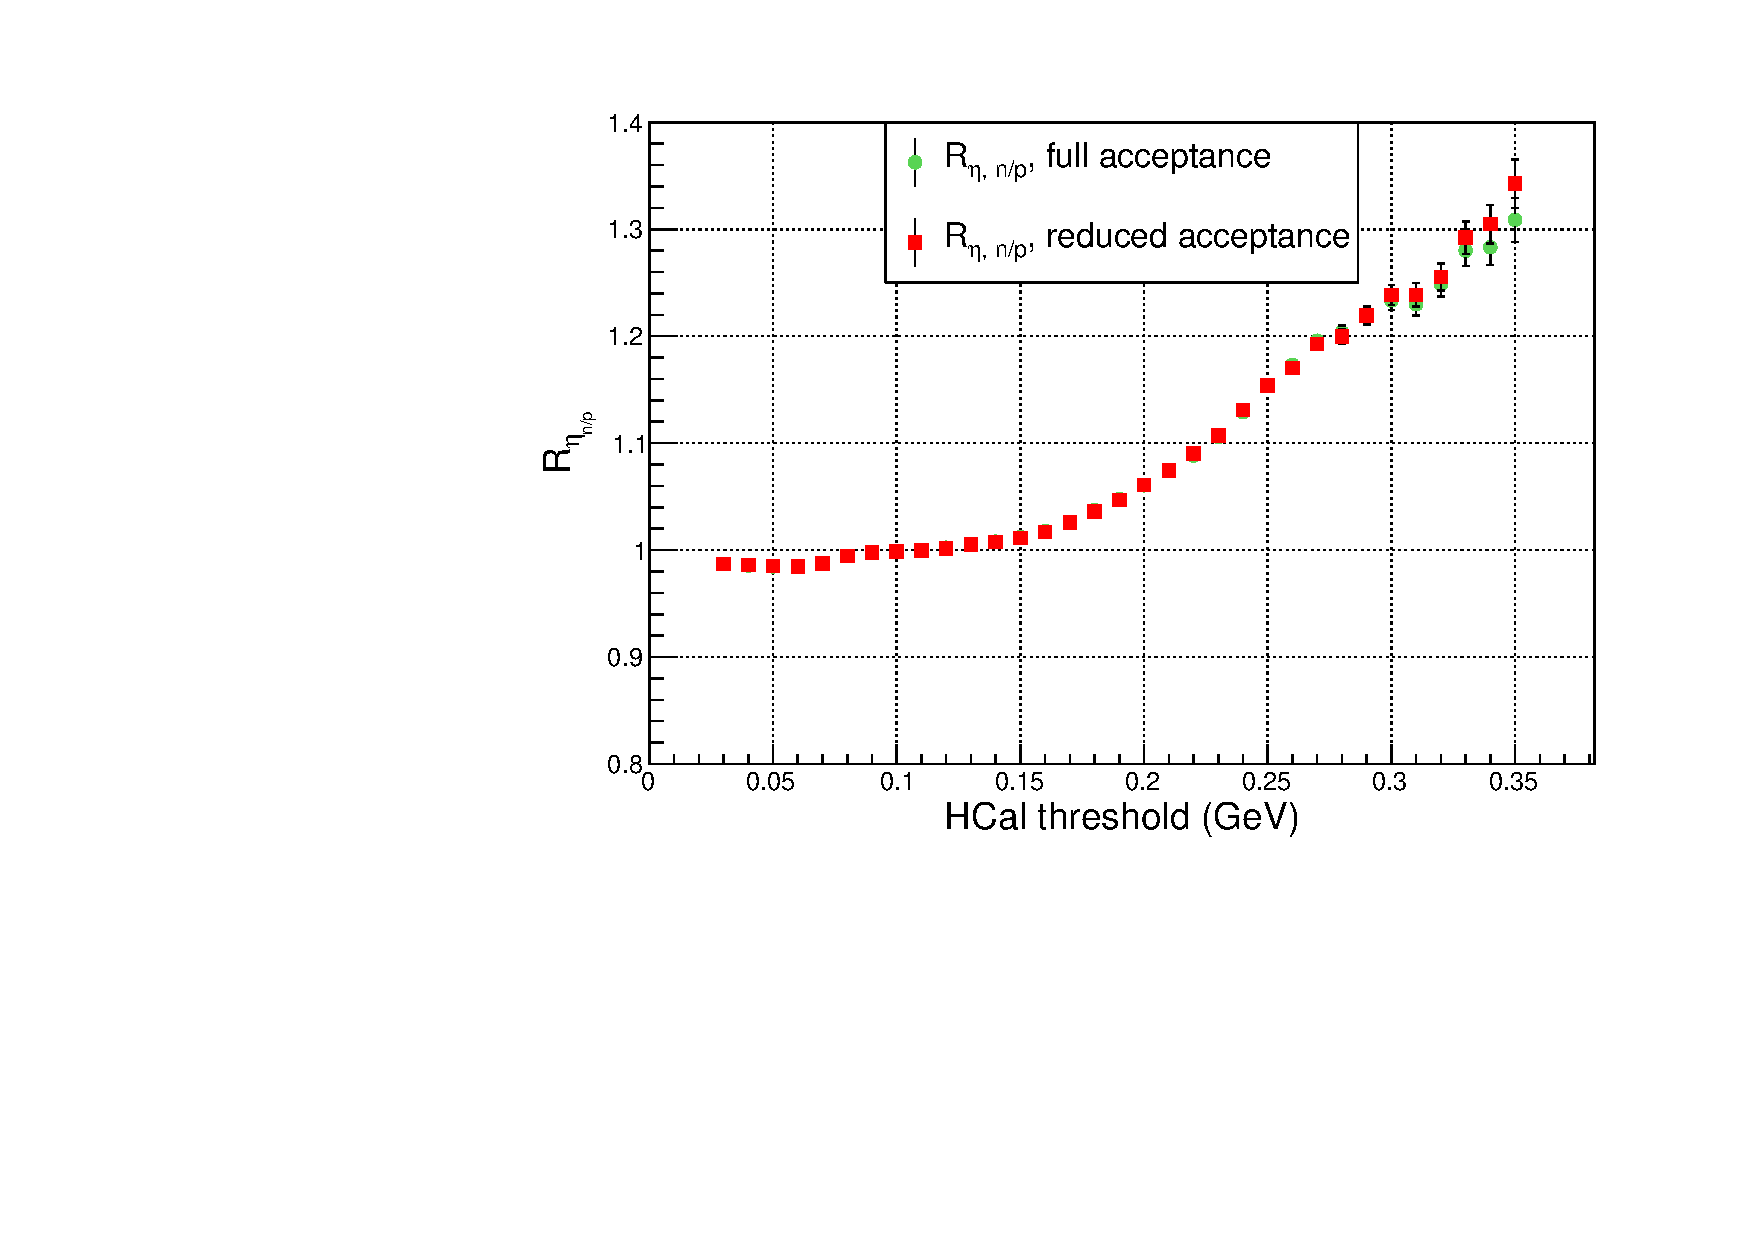
\includegraphics[width=7cm]{Reta_np_fthr_errs.pdf}
  \caption{Neutron/proton efficiency ratio $R_{\eta_{n/p}}$ as a function of the calorimeter threshold, for our quasi-elastic sample. The error bars represent the uncertainty from the calibration measurements discussed earlier. The green represents $R_{\eta_{n/p}}$ on the full acceptance, the red represents $R_{\eta_{n/p}}$ on a reduced acceptance.
    % The discrepancy between the two (blue) is about 0.1\% below a threshold of 0.15 GeV.%, but becomes about 0.5\% between 0.15 and 0.3 GeV, up to 1\% beyond 0.3 GeV}
  }
  \label{fig:Reta_np}
\end{figure}
%
$\Delta\eta_{p}$ and $\Delta\eta_{n}$ are the uncertainties from the calibration measurements described on the Monday write up. %$\sigma_{\eta-n/p}$. Fig~\ref{fig:Reta_np}.
The correlation between the variations of the proton and neutron efficiencies $\rho_{\eta_{n/p}}$, depends on the cause of the variations.
In the case of the efficiency calibrations runs, discussed in the Monday write-up,
the uncertainties of the efficiencies are due to the statistic of the collected events. 
In such a case, $\rho_{\eta_{n/p}} = 0$.
However, in the case of the detector instability, $\rho_{\eta_{n/p}} \sim 1$ (see again Fig.~\ref{fig:Reta_np}).

With the statistics projected for the calibration runs: $\eta_p \pm \Delta\eta_{p} = 0.915 \pm 0.003$ and $\eta_n \pm \Delta\eta_{n} = 0.924 \pm 0.014$.
Applying these values to Eq.~\ref{eq:uncert_exact}, %, and considering $R_{\eta_{n/p}} = 0.991$,
the relative uncertainty on the absolute value of the hadron efficiency ratio becomes:
%
\begin{equation}
  \Delta R_{\eta_{n/p}}/R_{\eta_{n/p}} = 1.6\%.
\end{equation}
%
Considering $R_{\eta_{n/p}} = 0.991$ from Fig.~\ref{fig:Reta_np}, $\Delta R_{n/p}/R_{n/p} = 0.016$. 
This would add up to the total systematic uncertainty of $R_{n/p}$ to 1.9\% for the low $\epsilon$ kinematic and to 1.6\% for the high $\epsilon$ kinematic.\\

However, %as it was demonstrated in Tuesday's write-up,
the measurement of the Rosenbluth slope, $S^n = \sigma_L/\sigma_T$, is unaffected by the uncertainty of the absolute value of the efficiency ratio $R_{\eta_{n/p}}$.
$R_{\eta_{n/p}}$ will be cancelled in the the determination of the neutron Rosenbluth slope $S^n$, 
{\it as long as we control the stability of $R_{\eta_{n/p}}$ over the few days of the measurement}.
%

\newpage

\subsection*{Efficiency stability due to the detector parameters drift}

As we know, the stability of the hadron detector efficiency is critical for a successful measurement.
The instability of the efficiency $\eta$ over time is mainly due to the drift of the PMTs signals and the related electronics.
Such an amplitude drift is typically of 1-2\% over a few days.
It will be better for our detector thanks to the LED calibration system.

We expect to use a threshold $A_{thr}$ = 100 MeV (see plots of amplitude spectrum in the Monday write-up).
Using the graph of the nucleon detection efficiency as a function of the threshold $A_{thr}$ on Fig.~\ref{fig:eta_N},
we find that, in the region $A_{thr} = 90 - 110$~MeV, the efficiency is:
%
\begin{equation}
  \eta = 0.92 - 0.18 \times \frac{A[{\rm MeV}]-100}{100}
\end{equation}
%
A one percent variation of $A_{thr}$ leads to 0.2\% variation of efficiency.
%
\begin{figure}[!h]
  \centering
  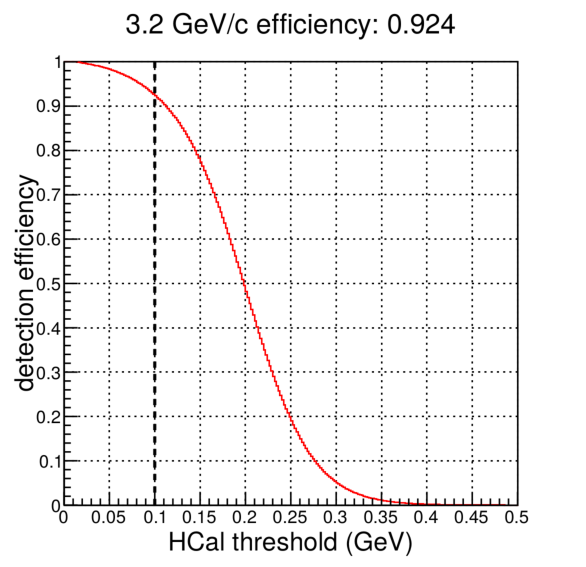
\includegraphics[width=7cm]{Neff_fThr.pdf}
  \caption{Nucleon detection efficiency vs the calorimeter threshold $A_{thr}$.}
  \label{fig:eta_N}
\end{figure}
%

Turning now to the ratio of efficiencies, we plot it as a function of the threshold on Fig.~\ref{fig:Reta_np}.
We find that, in the region $A_{thr} = 90 - 110$~MeV, the ratio of efficiencies is:
%
\begin{equation}
  R_{\eta_{n/p}} = \frac{\eta_n}{\eta_p} = 0.998 + 0.011 \times \frac{A[{\rm MeV}]-100}{100}.
\end{equation}
%
Using the estimate for a PMT-based system instability of 1-2\%, which means that $A_{thr}$ is stable to 1-2 MeV,
the ratio of efficiencies $R_{\eta_{n/p}} = \frac{\eta_n}{\eta_p}$ is found to be stable to 0.022\%.

The run plan of the GMn experiment (E12-09-019), which will run next summer,
has a provision of running on the hydrogen target multiple times with different fields in the SBS dipole,
allowing the study of the stability of individual modules of HCal.


\end{document}
